
\large{\textbf{Các ứng dụng của Seq2seq}} \\[0.2em]
Seq2seq tự nằm đằng sau nhiều hệ thống mà bạn phải sử dụng hằng ngày. Chẳng hạn, mô hình seq2seq hỗ trợ các ứng dụng
như Google Dịch, thiết bị hỗ trợ giọng nói và chatbot trực tuyến. Nói chung, các ứng dụng này bao gồm:

\begin{itemize}
    \item Dịch máy - một bài báo năm 2016 của Google cho thấy cách tiếp cận chất lượng dịch thuật mô hình seq2seq
    hoặc vượt qua tất cả các kết quả được công bố hiện tại.
        {\center{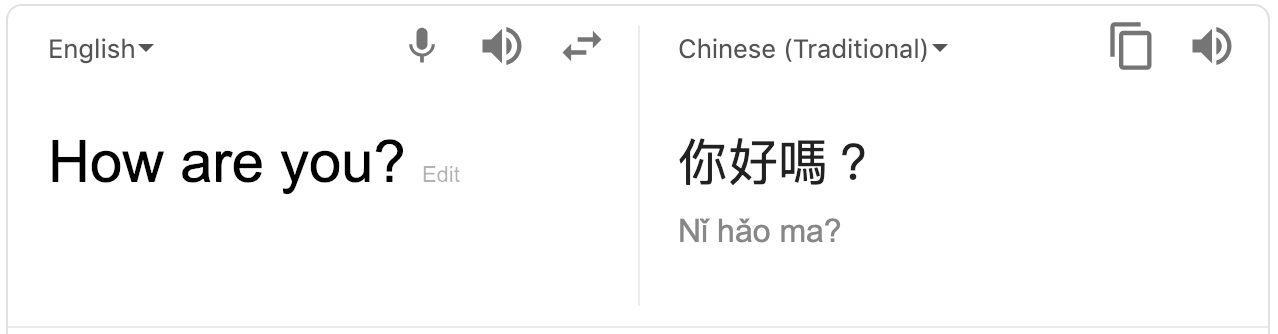
\includegraphics[width=\figureBigSize]{figure/model/SEQ-googletrans.png}}}
    \item Nhận dạng giọng nói - một bài báo khác của Google so sánh các mô hình seq2seq hiện có về nhiệm vụ nhận dạng
    giọng nói.
        {\center{
\includegraphics[width=\figureBigSize]{figure/model/SEQ-speech.png}}}
    \item Chú thích video - một bài báo năm 2015 cho thấy một seq2seq mang lại kết quả tuyệt vời như thế nào khi tạo
    mô tả phim.
        {\center{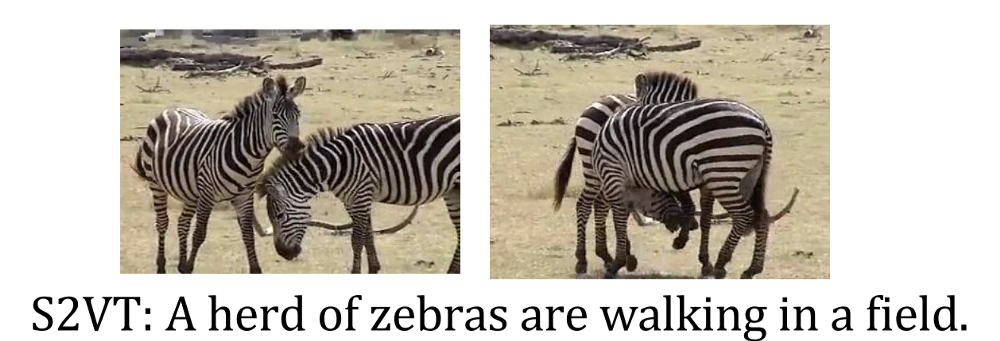
\includegraphics[width=\figureBigSize]{figure/model/SEQ-videocaption.png}}}
    \item Và đặc biệt tại Google I/O 2019 ,Google đã trình làng Translatotron, một công cụ cho phép dịch sang ngôn
    ngữ khác mà vẫn giữ được tông giọng của người nói
\end{itemize}

Đây chỉ là một số ứng dụng mà seq2seq được xem là giải pháp tốt nhất. Mô hình này có thể được sử dụng như một giải
pháp cho bất kỳ vấn đề dựa trên tuần tự nào, đặc biệt là các vấn đề đầu vào và đầu ra có dữ liệu khác nhau.

\large{\textbf{Cách Seq2seq hoạt động}} \\[0.2em]
Chúng ta sẽ xem qua hình minh họa ở dưới để hiểu cách hoạt động

\begin{figure}[!htb]
    \center{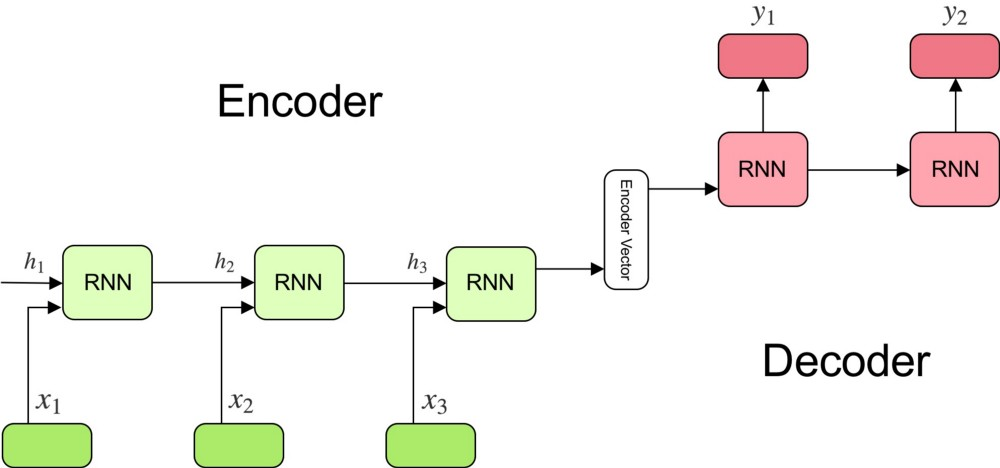
\includegraphics[width=\figureBigSize]
    {figure/model/SEQ-encoderdecoder.jpeg}}
    \caption{\label{fig:seq-encoderdecoder} Encoder-decoder seq2seq.}
\end{figure}

Model gồm 3 phần: encoder, intermediate (encoder) vector và decoder.

\textbf{Encoder}
\begin{itemize}
    \item Một chồng các đơn vị recurrent (các ô LSTM hoặc GRU để có hiệu suất tốt hơn) trong đó mỗi đơn vị tiếp
     nhận một phần tử duy nhất của chuỗi đầu vào, thu thập thông tin cho phần tử đó và đẩy nó về phía trước.
    \item Trong vấn đề chatbox, chuỗi đầu vào là tập hợp tất cả các từ trong câu đầu vào. Mỗi từ được biểu diễn
    dưới dạng \(x_i\) trong đó \(i\) là thứ tự của từ đó.
    \item Các trạng thái ẩn \(h_i\) được tính bằng công thức:
        \[h_t=f(W^{hh}h_{t-1} + W^{hx}x_t)\]
\end{itemize}
Công thức này đại diện cho kết quả của một Recurrent neural network thông thường. Có thể thấy, áp dụng
các trọng số phù hợp cho trạng thái ẩn trước đó \(h_{t-1}\) và vector đầu vào \(x_t\).

\textbf{Encoder Vector}
\begin{itemize}
    \item Đây là trạng thái ẩn cuối cùng được tạo ra từ phần \textbf{Encoder} của mô hình. Nó được tính bằng công thức trên.
    \item Vectoc này nhằm mục đích tổng hợp thông tin đầu vào để giúp \textbf{Decoder} đưa ra dự đoán chính xác.
    \item Nó hoạt động như trạng thái ẩn ban đầu của \textbf{Decoder} của model.
\end{itemize}

\textbf{Decoder}
\begin{itemize}
    \item Một chồng các đơn vị recurrent trong đó mỗi đơn vị dự đoán một đầu ra \(y_t\) tại một bước thời gian \(t\).
    \item Mỗi đơn vị định kỳ chấp nhận một trạng thái ẩn từ đơn vị trước đó và tạo ra và đầu ra cũng như trạng thái ẩn
    của chính nó.
    \item Trong vấn đề chatbot, chuỗi đầu ra là tập hợp tất cả các từ trong câu đáp. Mỗi từ được biểu diễn
    dưới dạng \(y_i\) trong đó \(i\) là thứ tự của từ đó.
    \item Bất kỳ trạng thái ẩn \(h_i\) nào cũng được tính bằng công thức:
        \[h_t=f(W^{hh}h_{t-1})\]
\end{itemize}
Như vậy có thế thấy rằng dùng trạng thái ẩn phía trước để tính trạng thái ẩn hiện tại
\begin{itemize}
    \item Đầu ra \(y_t\) tại bước thời gian \(t\) được tính bằng công thức:
        \[y_t=softmax(W^{s}h_{t})\]
\end{itemize}
Tính toán các đầu ra bằng cách sử dụng trạng thái ẩn ở bước thời gian hiện tại cùng với trọng số tương ứng
\(W(S)\). Softmax được sử dụng để tạo một vectoc xác suất sẽ giúp xác định đầu ra cuối cùng (ví dụ: từ
trong bài toán chatbot).

Sức mạnh của mô hình này nằm ở chỗ nó có thể ánh xạ các chuỗi có độ dài khác nhau với nhau. Như bạn có thể thấy đầu
vào và đầu ra không tương quan và độ dài của chúng có thể khác nhau. Điều này mở ra một loạt các vấn đề mới mà  bây
giờ có thể được giải quyết bằng kiến trúc như vậy.